\section{X : Algorithms III - Parsing and Grammars}
\label{chap:algos3}

%%%%%%%%%%%%%%%%%%%%%%%%%%%%%%%%%%%%%%%%%%%%%%%%%%%%%%%%%%%%%

\begin{frame}[fragile]
\frametitle{Parsing}
\begin{columns}[T]

\begin{column}{0.45\textwidth}
\begin{itemize}[<+->]
\item Several fundamental algorithms have been developed
to recognise legal computer programs (or expressions).
\item These decompose their structure into a form more suitable for processing.
\item This operation, know as parsing, has application
beyond Computer Science, since it is directly related to the study of
languages in general.
\item However, parsing human-friendly expressions is notoriously difficult.
\item Maybe we should write expressions in a machine-friendly way~?
\end{itemize}
\end{column}

\pause
\begin{column}{0.45\textwidth}
\begin{itemize}[<+->]
\item It is a long standing tradition in mathematics to write the operator
between the operands, as in \verb^x+y^, rather than \verb^x y +^.
\item The `normal' method with the operator between the operands is
known as {\it infix} notation.
\item As you scan a traditional infix expression, such as:
\begin{verbatim}
A+B/C+D
\end{verbatim}
from left- to right, it is impossible to tell when you initially encounter the \verb^+^ sign whether or not you should apply the indicated operation to
\item You need to worry about the `/' first since that has precedence. 
\end{itemize}
\end{column}

\end{columns}
\end{frame}


%%%%%%%%%%%%%%%%%%%%%%%%%%%%%%%%%%%%%%%%%%%%%%%%%%%%%%%%%%%%%

\begin{frame}[fragile]
\frametitle{Post-fix Notation (Reverse Polish)}
\begin{columns}[T]

\begin{column}{0.45\textwidth}
\begin{itemize}[<+->]
\item One must probe deeper into the expression to determine whether an operation with a higher priority occurs.
\item This gets very complicated.
\item Brackets make this even worse.
\item The alternative is called {\it Postfix} or {\it Reverse Polish}
after the Polish logician J.\ Lukasiewicz who investigated the
properties of this notation.
\end{itemize}
\end{column}

\begin{column}{0.45\textwidth}
\pause
Infix~:
\begin{verbatim}
A+B*C
A*B+C
((A+B)*C+D)/(E+F+G)
\end{verbatim}

Reverse Polish~:
\begin{verbatim}
ABC*+
AB*C+
AB+C*D+EF+G+/
\end{verbatim}

\pause
Notice that no brackets are required in Reverse Polish. Therefore, for
simple applications, we could require the user to enter expressions in
postfix form.
\end{column}

\end{columns}
\end{frame}

%%%%%%%%%%%%%%%%%%%%%%%%%%%%%%%%%%%%%%%%%%%%%%%%%%%%%%%%%%%%%%
\begin{frame}[fragile]
\frametitle{Implementing a Reverse Polish Parser}
\begin{columns}[T]

\begin{column}{0.45\textwidth}
\begin{itemize}[<+->]
\item Reverse Polish may be evaluated by use of a stack.
\item Examine the next character;
\item If it is a number (or variable in the general case)
push it onto the stack.
\item If it is an operator (+-/*), pop off the top two
items, perform the operation and push the result.
\item If we have reached the end the answer is the one and only
item on the stack. Else repeat.
\end{itemize}
\end{column}

\pause
\begin{column}{0.45\textwidth}
\begin{verbatim}
8 2 5 * + 1 3 2 * + 4 - /
\end{verbatim}
\begin{center}
\begin{tabular}{|c|c|c|c|c|c|c|c|c|}\hline
   & * & + &   & * & + & - &   & $/$ \\ \hline
   &   &   & 2 &   &   &   &   &     \\
 5 &   &   & 3 & 6 &   & 4 &   &     \\
 2 & 10&   & 1 & 1 & 7 & 7 & 3 &     \\
 8 & 8 & 18& 18& 18& 18& 18& 18& 6   \\ \hline
\end{tabular}
\end{center}
\end{column}

\end{columns}
\end{frame}

%%%%%%%%%%%%%%%%%%%%%%%%%%%%%%%%%%%%%%%%%%%%%%%%%%%%%%%%%%%%%%

\begin{frame}[fragile]
\frametitle{Coding a Postfix Parser}
\begin{columns}[T]

\begin{column}{0.55\textwidth}
\lstinputlisting[style=basicc,linerange={12-45},numbers=none]{../Code/ChapX/postfix.c}
\end{column}

\pause
\begin{column}{0.35\textwidth}
\outputlisting{../Code/ChapX/pfx1.manout}
\pause
\outputlisting{../Code/ChapX/pfx2.manout}
\pause
\outputlisting{../Code/ChapX/postfix.manout}
\end{column}

\end{columns}
\end{frame}

%%%%%%%%%%%%%%%%%%%%%%%%%%%%%%%%%%%%%%%%%%%%%%%%%%%%%%%%%%%%%%
\begin{frame}[fragile]
\frametitle{General Infix to Postfix}
\begin{columns}[T]

\begin{column}{0.45\textwidth}
{\footnotesize
www.geeksforgeeks.org/stack-set-2-infix-to-postfix
}

{\tiny
\begin{verbatim}
1. Scan the infix expression from left to right. 
2. If the scanned character is an operand, output it. 
3. Else, 
  1 If the precedence of the scanned operator is
    greater than the precedence of the operator
    in the stack(or the stack is empty  or the
    stack contains a '(' ), push it. 
  2 Else, Pop all the operators from the stack
    which are greater than or equal to in
    precedence than that of the scanned
    operator.  After doing that Push
    the scanned operator to the stack.  (If you
    encounter parenthesis while popping then stop
    there and push the scanned operator in the
    stack.) 
4. If the scanned character is an '(', push it to the
   stack. 
5. If the scanned character is an ')', pop the stack
   and and output it until a '(' is encountered, and
   discard both the parenthesis. 
6. Repeat steps 2-6 until infix expression is scanned. 
7. Print the output 
8. Pop and output from the stack until it is not
   empty.
\end{verbatim}
}
\end{column}

\pause
\begin{column}{0.45\textwidth}
{\tiny
\url{https://en.wikipedia.org/wiki/Shunting-yard_algorithm}
}
\begin{center}
\includegraphics[height=0.7\textheight]{../Images/Shunting_yard.png}
\end{center}
\end{column}

\end{columns}
\end{frame}


%%%%%%%%%%%%%%%%%%%%%%%%%%%%%%%%%%%%%%%%%%%%%%%%%%%%%%%%%%%%%%

\begin{frame}[fragile]
\frametitle{Formal Grammars}
\begin{columns}[T]

\begin{column}{0.40\textwidth}
\begin{itemize}[<+->]
\item Parsing a program is the process of grammatically analysing how it is composed into parts.
\item Before we can write a program to determine whether a program
written in a given language is legal, we need a description of exactly
what constitutes a legal program.
\item Programming languages are often described by a particular type of
grammar called a {\it context free grammar}.
\item You don't need to understand the input to check if it's valid or not.
\end{itemize}
\end{column}

\pause
\begin{column}{0.50\textwidth}
{\footnotesize
Based on : \verb^web.stanford.edu/class/archive/cs/cs143/cs143.1128^

\begin{verbatim}
<SENTENCE> ::= <SUBJECT> <VERB-PHRASE> <OBJECT>
<SUBJECT> ::= "This" | "Computers" | "I"
<VERB-PHRASE> ::= <ADVERB> <VERB> | <VERB>
<ADVERB> ::= "never"
<VERB> ::= "is" | "run" | "am" | "tell"
<OBJECT> ::= "the" <NOUN> | "a" <NOUN> | <NOUN>
<NOUN> ::= "university" | "world" | "cheese" | "lies"
\end{verbatim}

\pause
\begin{verbatim}
This is a university.
Computers run the world.
I am the cheese.
I never tell lies.
\end{verbatim}
}
\end{column}

\end{columns}
\end{frame}

%%%%%%%%%%%%%%%%%%%%%%%%%%%%%%%%%%%%%%%%%%%%%%%%%%%%%%%%%%%%%%

\begin{frame}[fragile]
\frametitle{A Formal Grammer : 0\&1s}
\begin{columns}[T]

\begin{column}{0.45\textwidth}
\begin{itemize}[<+->]

\item Say we wish to create a new computer language whose sole purpose
is to print out noughts and ones onto the screen~:

\pause
\begin{verbatim}
BEGIN
    ONE
    NOUGHT
    ONE
END
\end{verbatim}

\pause
\item The formal grammar : Backus-Naur form (BNF)~:
{\footnotesize
\begin{verbatim}
<PROG>      ::= "BEGIN" <CODE>
<CODE>      ::= "END" | <STATEMENT> <CODE>
<STATEMENT> ::= "ONE" | "NOUGHT"
\end{verbatim}
}
\end{itemize}

\end{column}

\pause
\begin{column}{0.45\textwidth}
{\small
\begin{itemize}[<+->]
\item The `\verb^|^' means OR.
\item \verb^"BEGIN"^, \verb^"ONE"^, \verb^"NOUGHT"^ and \verb^"END"^ are string constants.
\item \verb^<CODE>^ is described recursively.
\item You could also think of this grammar in terms of a {\it railroad diagram}:
\begin{center}
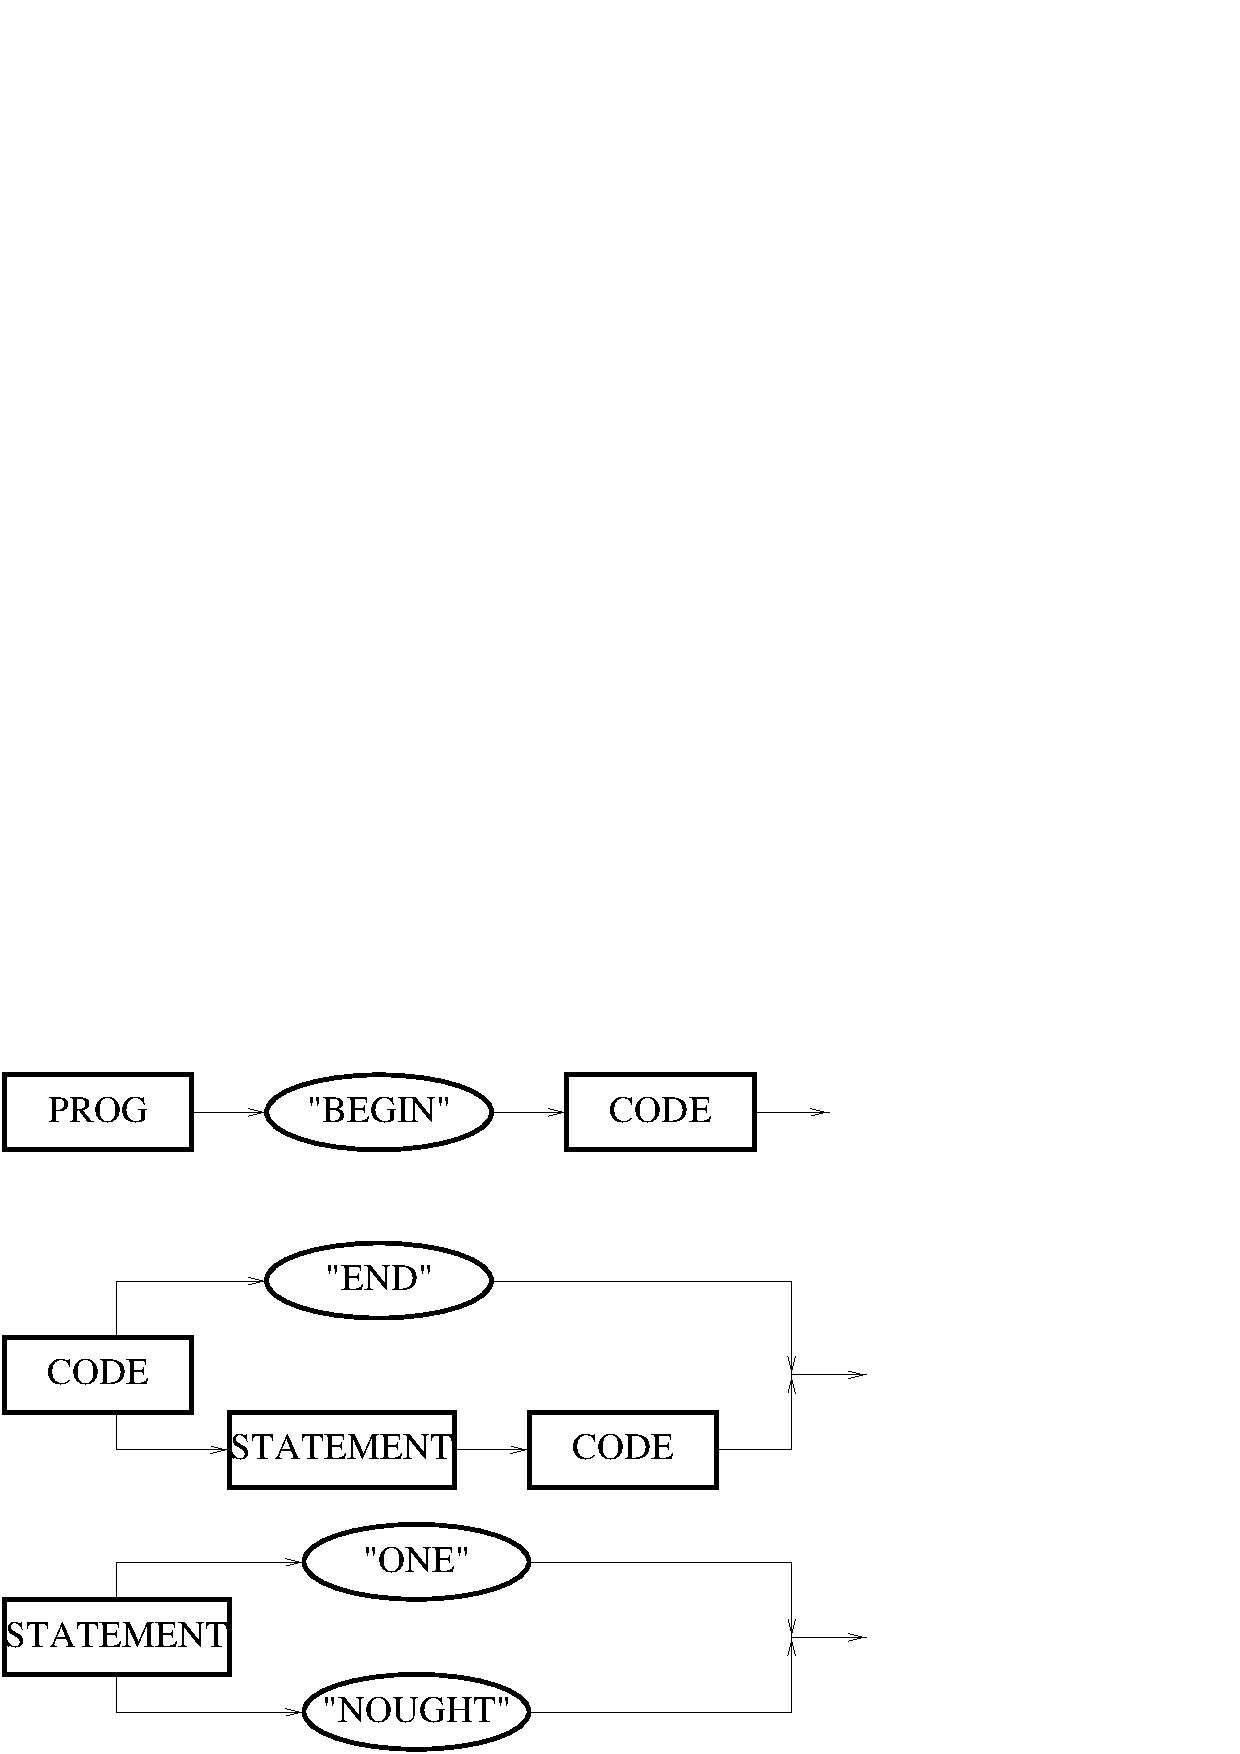
\includegraphics[width=0.5\textwidth]{../Images/railroad.pdf}
\end{center}
\end{itemize}
}
\end{column}

\end{columns}
\end{frame}


%%%%%%%%%%%%%%%%%%%%%%%%%%%%%%%%%%%%%%%%%%%%%%%%%%%%%%%%%%%%%%

\begin{frame}[fragile]
\frametitle{Coding a 0 \& 1s Parser}
\begin{columns}[T]

\begin{column}{0.55\textwidth}
\lstinputlisting[style=basicc,linerange={1-33}]{../Code/ChapX/0and1s.c}
\end{column}

\pause
\begin{column}{0.35\textwidth}
\lstinputlisting[style=basicc,linerange={35-63},numbers=none]{../Code/ChapX/0and1s.c}
\end{column}

\end{columns}
\end{frame}

%%%%%%%%%%%%%%%%%%%%%%%%%%%%%%%%%%%%%%%%%%%%%%%%%%%%%%%%%%%%%%

\begin{frame}[fragile]
\frametitle{Running the Parser}
\begin{columns}[T]

\begin{column}{0.45\textwidth}
{\tiny

\pause
{\bf
\begin{verbatim}
BEGIN
   ONE
   NOUGHT
   ONE
END
\end{verbatim}
}
\vspace*{-1.5ex}
Parsed OK

\pause
{\bf \begin{verbatim}
BEGIN ONE NOUGHT NOUGHT END
\end{verbatim} }
\vspace*{-1.5ex}
Parsed OK

\pause
{\bf \begin{verbatim}
BEGIN END
\end{verbatim} }
\vspace*{-1.5ex}
Parsed OK

\pause
{\bf \begin{verbatim}
BEGIN
  ONE
  TWO
END
\end{verbatim} }
\vspace*{-1.5ex}
Fatal Error Expecting a ONE or NOUGHT ?
occurred in p01a.c, line 79

\pause
{\bf \begin{verbatim}
BEGIN
  ONE
  NOUGHT
\end{verbatim} }
\vspace*{-1.5ex}
Fatal Error Expecting a ONE or NOUGHT ?
occurred in p01a.c, line 79

}
\end{column}


\pause
\begin{column}{0.45\textwidth}
{\tiny
{\bf \begin{verbatim}
  ONE
  NOUGHT
END
\end{verbatim} }
\vspace*{-1.5ex}
Fatal Error No BEGIN statement ?
occurred in p01a.c, line 55
}
\begin{itemize}[<+->]
\item Notice that the END statement is actually used as the recursive base-case in the formal grammar in the function Code().
\item The parser doesn't actually {\bf do} anything other than check that the input is {\bf valid} or not.
\item An interpreter performs the required operations (e.g. printing to the screen in this case) alongside the parser checking the syntax.
\item A slight modification to the code is required to produce an interpreter.
\end{itemize}
\end{column}

\end{columns}
\end{frame}

%%%%%%%%%%%%%%%%%%%%%%%%%%%%%%%%%%%%%%%%%%%%%%%%%%%%%%%%%%%%%%

\begin{frame}[fragile]
\frametitle{Interpreters are Modified Parsers}
\begin{columns}[T]

\begin{column}{0.45\textwidth}
\lstinputlisting[style=basicc,linerange={53-65},numbers=none]{../Code/ChapX/0and1s-interp.c}
\end{column}

\pause
\begin{column}{0.45\textwidth}
\outputlisting{../Code/ChapX/0and1s-interp.manout}
\pause
\begin{itemize}[<+->]
\item I've also taken out the "Parsed OK" message.
\item To extend the parser to be an interpreter you might now need to `understand' what the input means - the context-free requirement is removed somewhat.
\end{itemize}
\end{column}

\end{columns}
\end{frame}

%%%%%%%%%%%%%%%%%%%%%%%%%%%%%%%%%%%%%%%%%%%%%%%%%%%%%%%%%%%%%%

\begin{frame}[fragile]
\frametitle{Formal Grammar for Parsing Maths Expressions}

\begin{columns}[T]

\begin{column}{0.45\textwidth}
To parse a string such as:\\
"A+B*C"\\
"A*(B+C)" or\\
"-(B*F)"\\
we could invent our own grammar~:

\pause
\begin{verbatim}
<EXPR> ::= <EXPR><OP><EXPR> |
           "(" <EXPR> ")" |
           "-"<EXPR> | Letter
<OP>   ::= "+" | "-" | "*" | "/"
\end{verbatim}
\end{column}

\pause
\begin{column}{0.45\textwidth}
\lstinputlisting[style=basicc,linerange={1-33}]{../Code/ChapX/mathsexpr.c}
\end{column}

\end{columns}
\end{frame}


%%%%%%%%%%%%%%%%%%%%%%%%%%%%%%%%%%%%%%%%%%%%%%%%%%%%%%%%%%%%%%
\begin{frame}[fragile]
\frametitle{Running the Maths Parser}

\begin{columns}[T]

\begin{column}{0.45\textwidth}
\lstinputlisting[style=basicc,linerange={35-72},numbers=none]{../Code/ChapX/mathsexpr.c}
\end{column}


\pause
\begin{column}{0.45\textwidth}
\outputlisting{../Code/ChapX/mathsexpr.out1}
\pause
\outputlisting{../Code/ChapX/mathsexpr.out2}
\pause
\outputlisting{../Code/ChapX/mathsexpr.out3}
\end{column}

\end{columns}
\end{frame}


%%%%%%%%%%%%%%%%%%%%%%%%%%%%%%%%%%%%%%%%%%%%%%%%%%%%%%%%%%%%%%

\begin{frame}[fragile]
\frametitle{Running the Maths Parser}

\begin{columns}[T]

\begin{column}{0.45\textwidth}
\outputlisting{../Code/ChapX/mathsexpr.out4}
\pause
\outputlisting{../Code/ChapX/mathsexpr.out5}
\pause
\outputlisting{../Code/ChapX/mathsexpr.out6}
\end{column}

\pause
\begin{column}{0.45\textwidth}
\begin{itemize}[<+->]
\item The formal grammar doesn't explain everything that the
programmer needs to know.
\item It is not clear whether the \verb^a+c^ example is
invalid or not.
\item It is not clear how spaces should be dealt with.
\end{itemize}
\end{column}

\end{columns}
\end{frame}

%%%%%%%%%%%%%%%%%%%%%%%%%%%%%%%%%%%%%%%%%%%%%%%%%%%%%%%%%%%%%%
